%%% Template originaly created by Karol Kozioł (mail@karol-koziol.net) and modified for ShareLaTeX use

\documentclass[a4paper,11pt]{article}

\usepackage[utf8]{inputenc}
\usepackage{graphicx}
\usepackage{xcolor}

\usepackage{tgheros}
%\usepackage[defaultmono]{droidmono}

\usepackage{amsmath,amssymb,amsthm,textcomp}
\usepackage{enumerate}
\usepackage{multicol}
\usepackage{tikz}

\usepackage{geometry}
\geometry{total={210mm,297mm},
left=25mm,right=25mm,%
bindingoffset=0mm, top=20mm,bottom=20mm}


\linespread{1.3}

\newcommand{\linia}{\rule{\linewidth}{0.5pt}}

% custom theorems if needed
% my own titles
\makeatletter
\renewcommand{\maketitle}{
\begin{center}
\vspace{2ex}
{\huge \textsc{\@title}}
\vspace{1ex}
\\
\linia\\
\@author \hfill \@date
\vspace{4ex}
\end{center}
}
\makeatother
%%%

% custom footers and headers
\usepackage{fancyhdr}
\pagestyle{fancy}
\lhead{}
\chead{}
\rhead{}
\lfoot{ADE:Assignment 1}
\cfoot{Page \thepage}
\rfoot{15M54097}
\renewcommand{\headrulewidth}{0pt}
\renewcommand{\footrulewidth}{0pt}
%

% code listing settings
\usepackage{listings}
\lstset{
    language=SQL,
    basicstyle=\ttfamily\small,
    aboveskip={1.0\baselineskip},
    belowskip={1.0\baselineskip},
    columns=fixed,
    extendedchars=true,
    breaklines=true,
    tabsize=4,
    prebreak=\raisebox{0ex}[0ex][0ex]{\ensuremath{\hookleftarrow}},
    frame=lines,
    showtabs=false,
    showspaces=false,
    showstringspaces=false,
    keywordstyle=\color[rgb]{0.627,0.126,0.941},
    commentstyle=\color[rgb]{0.133,0.545,0.133},
    stringstyle=\color[rgb]{01,0,0},
    numbers=left,
    numberstyle=\small,
    stepnumber=1,
    numbersep=10pt,
    captionpos=t,
    escapeinside={\%*}{*)}
}

%%%----------%%%----------%%%----------%%%----------%%%

\begin{document}

\title{Advanced Data Engineering: Assignment 1}

\author{NGUYEN T. Hoang - SID: 15M54097}

\date{Fall 2015, W831 Tue. Period 5-6 \\ \hfill Due date: 2015/10/20}

\maketitle

\vfill

\section*{Problem}

Consider 4 relations:
\begin{itemize}
    \setlength{\itemsep}{0cm}
    \setlength{\parskip}{0cm}
    \item \textbf{Products} (ProductID, ProductName, ProductType, Price)
    \item \textbf{Categories} (ProductType, Category)
    \item \textbf{ShopA} (ProductID, Stocks)
    \item \textbf{ShopB} (ProductID, Stocks)
\end{itemize}
\vfill
\section*{Question 1}

\textit{Write a SQL query to derive ``ProductName'' and ``Price'' of product categorized as ``Printer'', of which ShopA or ShopB keeps more than five stocks.} 

\noindent
\textbf{Answer:} \\[-3em]

\begin{lstlisting}[label={list:first},caption=SQL query to get 'Printer' product with more than 5 stocks in ShopA or ShopB]
SELECT P.ProductName, P.Price
FROM Products P
WHERE 
    P.ProductType IN (
        SELECT C.ProductType
        FROM Categories C
        WHERE C.Category = 'Printer')
    AND 
    (P.ProductID IN (
        SELECT A.ProductID
        FROM ShopA A
        WHERE Stocks > 5)
    OR P.ProductID IN (
        SELECT B.ProductID
        FROM ShopB B
        WHERE Stocks > 5)
    );
\end{lstlisting}
\vfill
\pagebreak

\vspace*{3em}

\section*{Question 2}

\textit{Express the same query in Relational Algebra and draw a query tree for the expression.}

\noindent
\textbf{Answer:} 
\noindent
The Relational Algebra expression equivalent with the query in \emph{Listing 1} is given as follow:

\vspace{1.5em}

\hline

\begin{center}

\Pi_{
    \begin{subarray}{l}
        \text{P.ProductName}, \\
        \text{P.Price}\\
    \end{subarray}
}
\big(\big(
\Pi_{
    \begin{subarray}{l}
        \text{P.ProductID},\\
        \text{P.ProductName},\\
        \text{P.Price}\\
    \end{subarray}
}
\sigma_{
    \begin{subarray}{l}
        \text{P.ProductType = C.ProductType} \\ \land 
        \text{ C.Category = 'Printer'}\\
    \end{subarray}
}
\big( \rho_P(\text{Products}) \times \rho_C(\text{Categories}) \big) \big) \\
\Join
\big(
\Pi_{
    \begin{subarray}{l}
        \text{A.ProductID}\\
    \end{subarray}
}
\sigma_{
\begin{subarray}{l}
\text{Stocks \textgreater \ 5 }\\
\end{subarray}
}
\rho_A(\text{ShopA})
\cup
\Pi_{
    \begin{subarray}{l}
        \text{B.ProductID }\\
    \end{subarray}
}
\sigma_{
\begin{subarray}{l}
\text{Stocks \textgreater \ 5 }\\
\end{subarray}
}
\rho_B(\text{ShopB})
\big)
\big)

\end{center}

\hline

\vspace{1em}
\noindent
The equivalent query tree:
\begin{figure}[htbp]
    \centering
    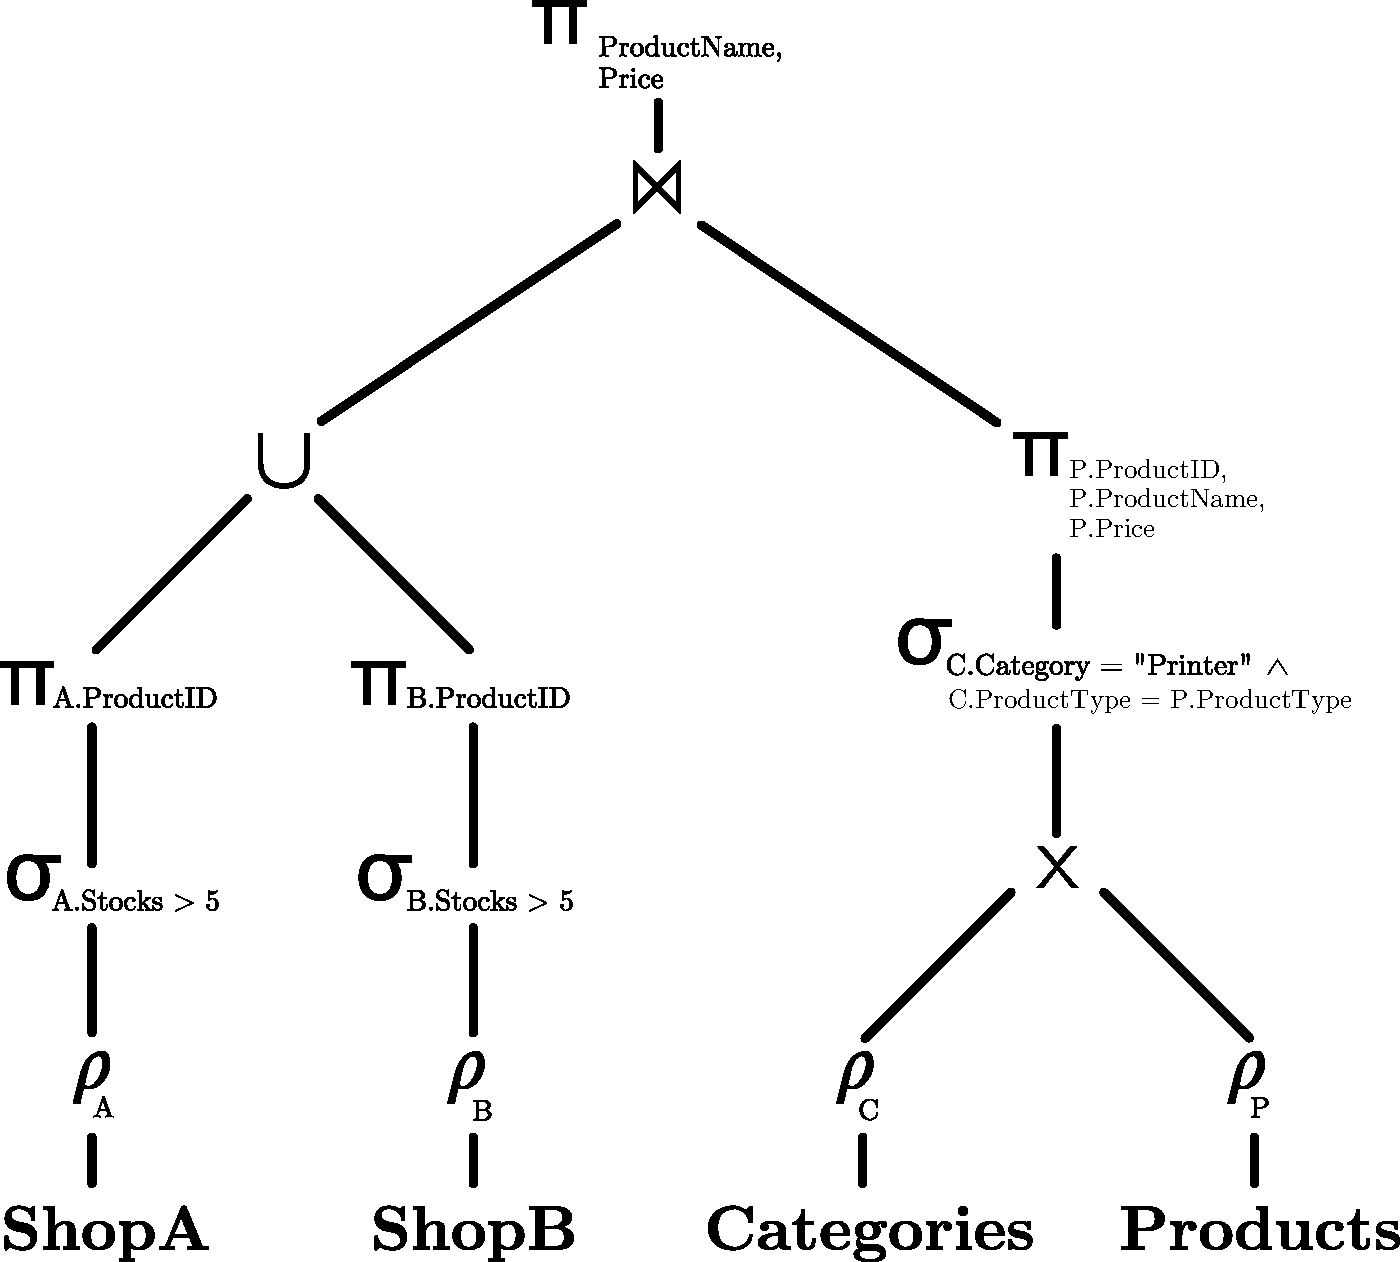
\includegraphics[scale=0.5]{ADE_A1_QueryTree.pdf}
    \caption{Query Tree for ProductName and Price of all `Printer'}
\end{figure}



\pagebreak

\section*{Question 3}

\textit{Write an SQL query to derive maximum price of each product type of products sold in both ShopA and ShopB with ``ProductType'' and ``Category''.} 

\noindent
\textbf{Answer:} \\[-3em]

\begin{lstlisting}[label={list:first},caption=SQL query to return maximum price for each categories.]
SELECT P.ProductType, C.Category, Max(P.Price) AS MaxPrice
FROM Products P, Categories C
WHERE 
    P.ProductID IN (
        SELECT ProductID
        FROM ShopA)
    AND P.ProductID IN (
        SELECT ProductID 
        FROM ShopB) 
    AND P.ProductType = C.ProductType
    GROUP BY P.ProductType;
\end{lstlisting}

\section*{Question 4}

\textit{Write an SQL query to derive ``ProductType'' and its ``Category'' of products sold in both ShopA and ShopB, where the maximum price of the product type is less than 1000.} 

\noindent
\textbf{Answer:} \\[-3em]

\begin{lstlisting}[label={list:first},caption=Query for ProductType and Category pair that has maximum price less than 1000.] 
SELECT P.ProductType, C.Category
FROM Products P, Categories C
WHERE 
    P.ProductID IN (
        SELECT ProductID
        FROM ShopA)
    AND P.ProductID IN (
        SELECT ProductID 
        FROM ShopB) 
    AND P.ProductType = C.ProductType
    GROUP BY P.ProductType;
    HAVING MAX(P.Price) < 1000;
\end{lstlisting}


\end{document}
